%!TEX root = ../Thesis.tex

\chapter{Evaluation and optimization}
	\label{evaluation}
	During the course of creating the application we tried different approaches to several interim steps. In this chapter we discuss how using different algorithms yielded different results.

	\section{Dataset}
	\label{evaluation-dataset}
	In order to test and optimize our detector we created a set of 101 images and annotated them manually with the following information: each intersection on the board was tagged. Either as an empty intersection, an intersection with a white piece on it or one occupied by a black piece. Also, the location of all pieces was marked with a circle, i.e. with a center and an approximate radius.

	To have an image set that covers many possible game situations we took pictures in three different lighting conditions and on different backgrounds. Each time we took images of an empty board without any pieces, a board with only some few images and a configuration like it often happens during endgame. That is, many pieces on the board and lots of them in a line.

	Each board configuration was photographed from different angles in $\varphi$ (azimuth) and $\theta$ (polar) direction and from two directions, i.e. facing the board from the side a player would and rotated by 90\textdegree\ as a third person would see the board.

	\begin{figure}
		\begin{subfigure}[b]{0.3\textwidth}
			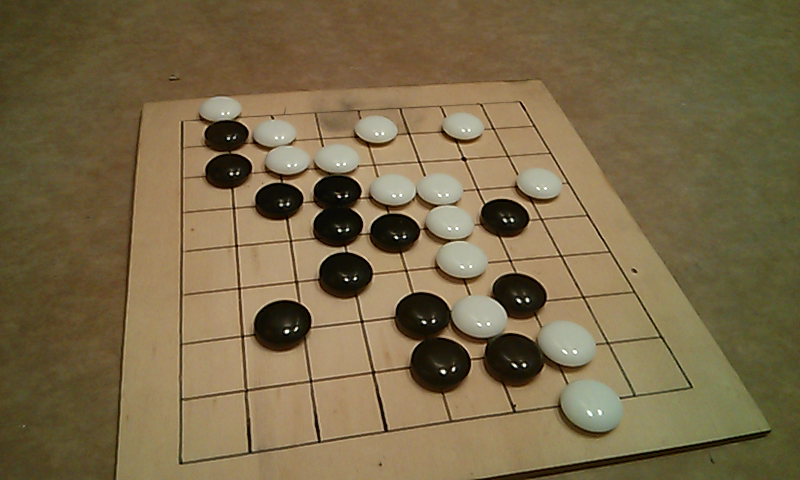
\includegraphics[width=\textwidth]{images/warmLight_many_leftMedium.png}
			\caption{Paper in warm light; camera left on medium height}
		\end{subfigure}
		~
		\begin{subfigure}[b]{0.3\textwidth}
				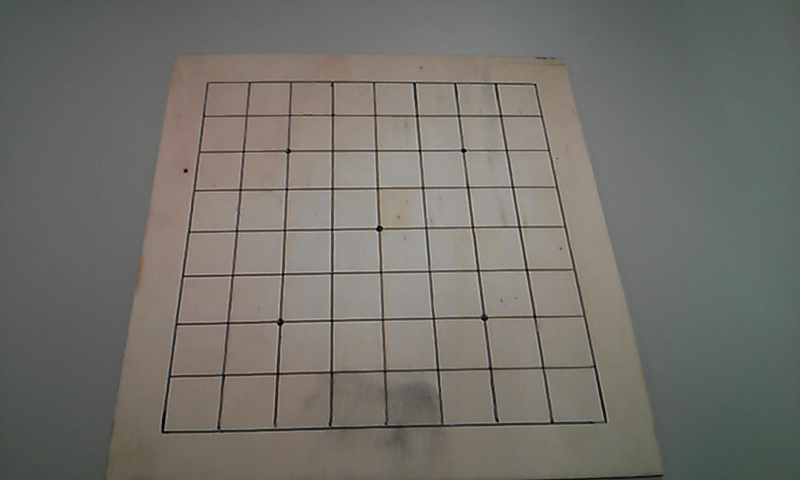
\includegraphics[width=\textwidth]{images/neonDesk_empty_centerAbove.png}
				\caption{Plain gray desk in neon light; camera centered high}
		\end{subfigure}
		~
		\begin{subfigure}[b]{0.3\textwidth}
				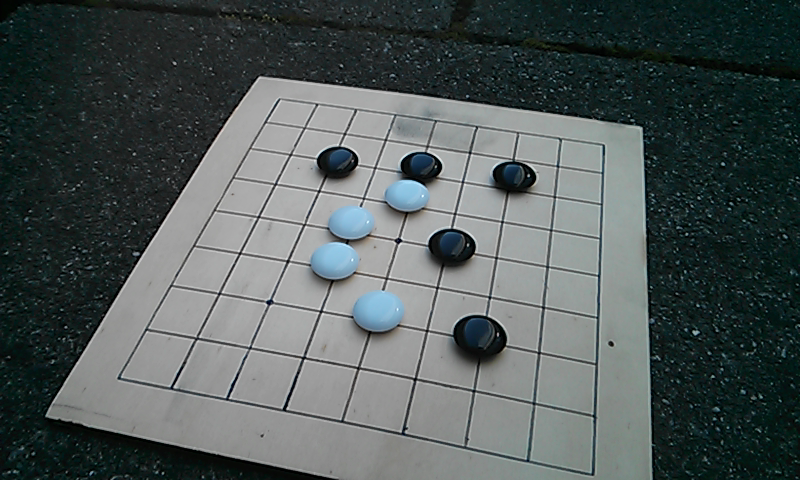
\includegraphics[width=\textwidth]{images/shadowStone_some_rightAbove.png}
				\caption{Dark stone surface in the shadow; camera right high}
		\end{subfigure}
		\\
		\begin{subfigure}[b]{0.3\textwidth}
				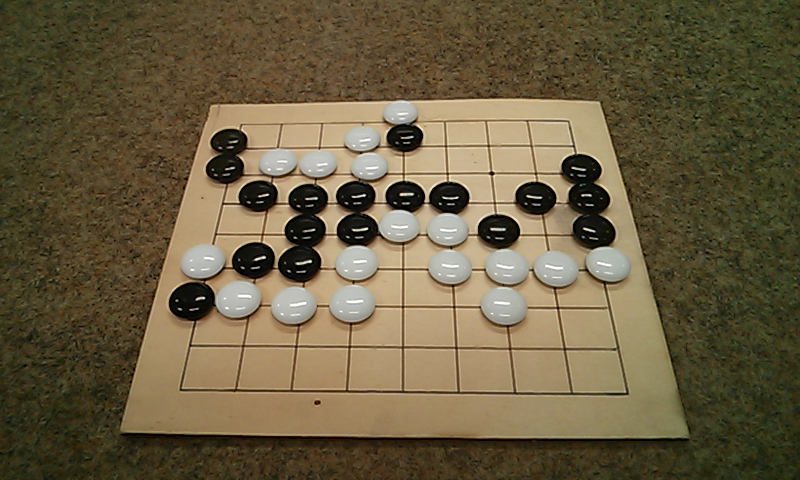
\includegraphics[width=\textwidth]{images/neonFloor_many_centerLow.png}
				\caption{Brown carpet in neon light; camera centered low}
		\end{subfigure}
		~
		\begin{subfigure}[b]{0.3\textwidth}
				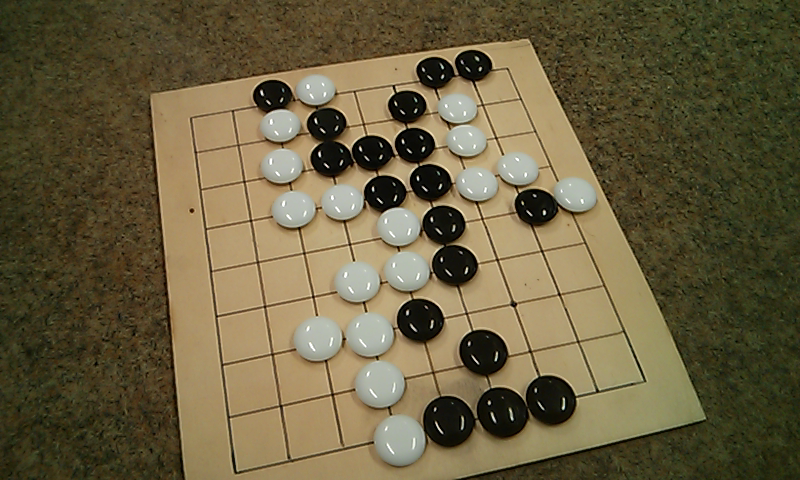
\includegraphics[width=\textwidth]{images/neonFloor_many_centerLow_rotated.png}
				\caption{Like (d) but from bystanders'	 perspective}
		\end{subfigure}
		~
		\begin{subfigure}[b]{0.3\textwidth}
			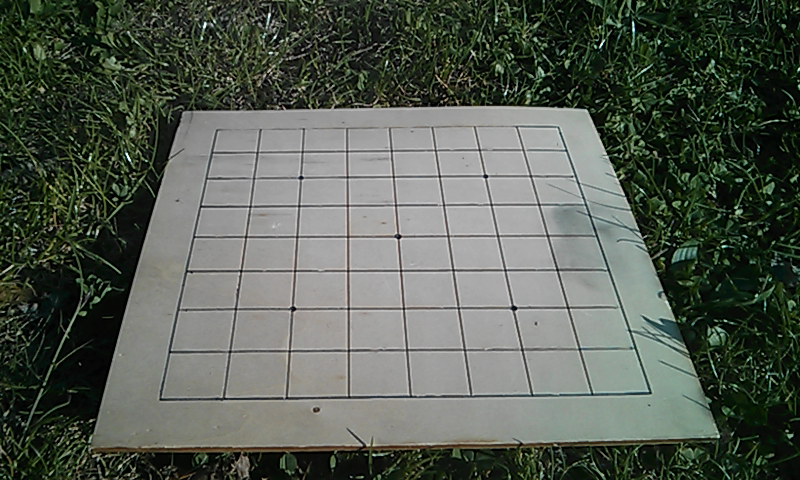
\includegraphics[width=\textwidth]{images/sunnyGrass_empty_centerLow.png}
			\caption{On grass in sunlight; camera centered low}
		\end{subfigure}

		\caption{Some examples of different lighting conditions, angles and backgrounds as well as different piece count}
		\label{fig:sampeImages}
	\end{figure}

	Our set consists of: 29 images taken in cold neon light on a plain gray desk; 26 images taken in the same light on a textured, brown carpet; 25 images taken on a sunny day in the shadow on a stone surface; 17 images in warm artificial light on a textured paper background. Furthermore we have taken 5 images in the sun on an evening while the board lay in grass. See \autoref{fig:sampeImages} for some examples from the image set\footnote{Our image set can be downloaded from http://t-animal.de/projects/bachelorThesis/ TODO}.

	The images were recorded by starting the app normally. But instead of calling the detector the input image was saved on the internal memory of the device. We did not take images using a camera or camera app to stay as close to the expectable input as possible.

	While in the beginning we saved images to PNG we later switched to persisting the images into yml format and retook the previous images. This has the advantage that we can be absolutely sure that the input to our test instances is the same as is would be on a phone, as no PNG encoding and decoding takes place. Also we first had problems because the OpenCV for Android function which persists images in PNG format presumably does not recognize that the camera image is encoded in RGB (see \autoref{android-detector}). This lead to different results on our desktop hardware than on our Android device.

	31 of the images were randomly chosen as a test set evenly spread over all lighting conditions as well as piece and angle configurations. The grass images with pieces on the board were not part of the test set as they soon turned out to be very difficult. We included them in the training set, though. This set was used to improve our detector.

	To do so we assumed that there is a global maximum for the overall quality of results when adjusting parameters of the used algorithms. Even if this assumption were wrong we optimized for a local maximum. Then we tried to manually find optimal parameters for some randomly chosen images for every algorithm. When we were contempt and could not find parameter combinations which yielded better results on the few images we fine tuned them on all training images. For this we automatedly created every combination of parameters in the vicinity of our manually optimized ones. Then we checked the results of those combinations on every image by brute force on a cluster of 45 oktacore machines. We compared the results to the annotations and transfered the best performing parameters into our application.






	\section{Visible intersections}
	\label{evaluation-visible}
	%TODO: eigentlich ist visible intersections falsch, weil ja auch unsichtbare gematcht werden
	When evaluating the detection rate of visible intersections we first checked if the intersection was within the boundaries of the annotated board and a padding of 15 pixels. If not the intersection was considered uninteresting and did neither count positively nor negatively (we assumed it to be noise outside the board). If it was inside the board we searched for the nearest annotated intersection. If there was none within a range of 15 pixels the intersection was counted as a false positive. But if there was, then the annotated intersection was marked as detected and not considered as a possible match for other intersections. The threshold of 15 pixels was chosen roughly as a quarter of the average distance between two intersections and a third of the diameter of a piece as measured in some sample images.

	%!TEX root = ../Thesis.tex

\begin{figure}
	\pgfplotsset{width=\textwidth, height=5.5cm, compat=1.11}
	\begin{subfigure}{\textwidth}
		\begin{tikzpicture}
			\begin{semilogyaxis}[
				ylabel={Intersections count},
				xlabel={Different parameter combinations},
				xtick style={draw=none},
				xticklabels={,,},
				axis x line=bottom,
				axis y line=left,
				legend style={at={(1,0.05)}, anchor=south east},
				xmin=0,
				ymin=0,
				xmax=610,
				ymax=6000
				]
				\draw[white!70!black, thin] ({rel axis cs:1,0}|-{axis cs:0,5670}) -- ({rel axis cs:0,0}|-{axis cs:0,5670});
				\draw[white!70!black, thin] ({rel axis cs:1,0}|-{axis cs:0,70}) -- ({rel axis cs:0,0}|-{axis cs:0,70});
				\draw[orange, thick] ({axis cs:381,5000}) -- ({axis cs:381,0}|-{rel axis cs:0,0});
				\draw[orange, thick] ({axis cs:0,5000}) -- ({axis cs:381,5000});

				\addplot[color=red, smooth]          table[x expr=\coordindex+1, y=matched, mark=none] {plots/lines_hough_part.csv};
				\addplot[color=red!40!black, smooth] table[x expr=\coordindex+1, y=wrong, mark=none] {plots/lines_hough_part.csv};

				\addlegendentry{Sum of true positives on all images}
				\addlegendentry{Sum of all false positives on all images}
			\end{semilogyaxis}
		\end{tikzpicture}
		\vspace{-20pt}
		\caption{Representative subset of 605 combinations of 60481 tested for the Houghline detector}
		\label{fig:linesTraining-hough}
	\end{subfigure}
	\vspace{20pt}

	\begin{subfigure}{\textwidth}
		\begin{tikzpicture}
			\begin{semilogyaxis}[
				ylabel={Intersections count},
				xlabel={Different parameter combinations},
				xtick style={draw=none},
				xticklabels={,,},
				axis x line=bottom,
				axis y line=left,
				legend style={at={(1,0.05)}, anchor=south east},
				xmin=0,
				ymin=0,
				xmax=610,
				ymax=6000
				]
				\draw[white!70!black, thin] ({rel axis cs:1,0}|-{axis cs:0,5670}) -- ({rel axis cs:0,0}|-{axis cs:0,5670});
				\draw[white!70!black, thin] ({rel axis cs:1,0}|-{axis cs:0,70}) -- ({rel axis cs:0,0}|-{axis cs:0,70});
				\draw[orange, thick] ({axis cs:158,1175}) -- ({axis cs:158,0}|-{rel axis cs:0,0});
				\draw[orange, thick] ({axis cs:0,1175}) -- ({axis cs:158,1175});

				\addplot[color=blue, smooth]          table[x expr=\coordindex+1, y=matched, mark=none, smooth,] {plots/lines_lsd_part.csv};
				\addplot[color=blue!40!black, smooth] table[x expr=\coordindex+1, y=wrong, mark=none, smooth, blue] {plots/lines_lsd_part.csv};

				\addlegendentry{Sum of true positives on all images}
				\addlegendentry{Sum of all false positives on all images}
			\end{semilogyaxis}
		\end{tikzpicture}
		\vspace{-20pt}
		\caption{Representative subset of 605 combinations of 58321 tested for the LSD detector.}
		\label{fig:linesTraining-lsd}
	\end{subfigure}
	\vspace{20pt}

	\begin{subfigure}{\textwidth}
		\begin{tikzpicture}
			\begin{semilogyaxis}[
				ylabel={Intersections count},
				xlabel={Different parameter combinations},
				xtick style={draw=none},
				xticklabels={,,},
				axis x line=bottom,
				axis y line=left,
				legend style={at={(1,0.05)}, anchor=south east},
				xmin=0,
				ymin=0,
				xmax=610,
				ymax=15000
				]
				\draw[white!70!black, thin] ({rel axis cs:1,0}|-{axis cs:0,5670}) -- ({rel axis cs:0,0}|-{axis cs:0,5670});
				\draw[white!70!black, thin] ({rel axis cs:1,0}|-{axis cs:0,70}) -- ({rel axis cs:0,0}|-{axis cs:0,70});
				\draw[orange, thick] ({axis cs:117,215}) -- ({axis cs:117,0}|-{rel axis cs:0,0});
				\draw[orange, thick] ({axis cs:0,215}) -- ({axis cs:117,215});

				\addplot[color=green, smooth]          table[x expr=\coordindex+1, y=matched, mark=none, smooth,] {plots/intersects_fast_part.csv};
				\addplot[color=green!40!black, smooth] table[x expr=\coordindex+1, y=wrong, mark=none, smooth, blue] {plots/intersects_fast_part.csv};

				\addlegendentry{Sum of true positives on all images}
				\addlegendentry{Sum of all false positives on all images}
			\end{semilogyaxis}
		\end{tikzpicture}
		\vspace{-20pt}
		\caption{Representative subset of 605 combinations of 1440 tested for the FAST detector}
		\label{fig:linesTraining-fast}
	\end{subfigure}

	\caption{The x-axis shows different combinations of parameters that we have evaluated. On the y-axis the true positives, false positives, totally available intersections (upper gray line) and number of analyzed images (lower gray line) per combination can be seen. The x-axis does not imply any order of the tested combinations; results have been simply sorted after number of correct intersections. We chose the parameter combination with the highest true positive rate whilst less false positives than evaluated files (orange line)}
	\label{fig:linesTraining}
\end{figure}


	\subsection{Optimizations on the training set}
	\label{evaluation-visible-optimization}
	While optimizing the parameters used in our algorithm, we measured the quality as the ratio of detected to undetected intersections, also considering the number of false positives. Traditionally one would calculate some ratio of true positives to false positives. However none of the usual measurement methods showed us a clear indication which combination of parameters to use, so we devised the following metric: We sorted the results by the number of correctly matched intersections from low to high. Then we chose the last one where the number of false positives was lower or equal than the number of images analyzed ($|false\_positives| \leq |input\_images|$, i.e., statistically maximal one false positive per image). This is shown (albeit on a representative subset of all tested parameter combinations) in \autoref{fig:linesTraining}, where the parameters we chose is marked in orange.

	\subsubsection{HOUGH}
	\label{evaluation-visible-optimization-hough}
	In comparison to the other algorithms detecting the lines using Hough transformation performs best quality-wise. As \autoref{fig:linesTraining-hough} shows, we still had to compromise when choosing the final parameter set. The one we chose resulted in 89.67\% (5084 out of 5670) correct detection rate on our training set, with a total of 68 incorrect intersections (1.199\% of available intersections).

	The graphic shows also, that the quality of the line detection does not depend very much on the parameters used: there's only a few parameter combinations that yield very poor results and hardly any that results in finding no intersection at all. This is generally a good thing, because it means that even if we chose a combination that is non-optimal under some circumstances its result quality does not collapse completely.

	As would be expected the average number of false positives rises with the percentage of correctly found intersections. Luckily, there is enough variance that even at a high detection rate we can find parameter combinations with less than one false intersection per image on average.

	\subsubsection{LSD}
	\label{evaluation-visible-optimization-lsd}
	As noted in \autoref{detector-visible-lsd} the Line Segment Detector needs significant postprocessing to give any reasonable results. Still it is easily outperformed by the variant using Hough transformation. In \autoref{fig:linesTraining-lsd} one can see that the amount of false positives does not drop below the number of input images for any parameter combination yielding more than about 25\% detection rate. Furthermore the average ratio of correct results to false positives is nearly all the time worse than its Hough counterpart's. Only in the rightmost segment the ratio is better. The total number of wrong intersections ranges in the thousands here, though, making this segment unusable for the application.

	The chosen parameter combination performs at a detection rate of only 20.53\% (1164 out of 5670) with 69 false positives. To achieve a detection rate similar to the one of the Hough detector we would have to accept more than 10 false positives per image on average.

	\subsubsection{FAST}
	\label{evaluation-visible-optimization-fast}
	The last tested algorithm is the FAST coner detector. It performs even worse when used for detection of the intersections. It is the only detector that resulted in more false positives than correct intersections in some combination. The ratio of false positives to correctly classified intersections is never better than the one line intersections detected by LSD or Hough transformation.

	The chosen parameter combination yields a mere 2.7\% (155 out of 5670) correctly detected intersections with 70 wrongly placed ones. Overall the detector seems to stick too much to the lines themselves and places many keypoints around them and at the border of the black pieces.

	\subsection{Performance on the testing set}
	\label{evaluation-visible-performance}
	To evaluate the performance of the three possible approaches we tested them on some images which had not been included in the training set.

	\begin{table}[b!]
		\begin{tabular}{lrc>{\bfseries}ccc}
		    \multicolumn{2}{c}{}									&\hphantom{Abst} & Hough 	& LSD 		& FAST     \\

			\toprule
			\multirow{2}{*}{No pieces on the board}   		& True positive rate 	&& 100\%	& 30.3\%  	& 0.685\%  \\
			%
															& Precision			 	&& 99.4\% 	& 94.2\%  	& 83.3\%  \\
			%																					  245/260	  5/6
			\midrule
			\multirow{2}{*}{Some pieces (7-13)}				& True positive rate 	&& 95.6\% 	& 11.4\% 	& 1.97\%   \\
			%
															& Precision 			&& 98.6\% 	& 91.2\%  	& 53.3\%  \\
			%																					  114/125	  16/30
			\midrule
			\multirow{2}{*}{Many pieces (27-34)} 			& True positive rate 	&& 58.6\% 	& 9.02\% 	& 3.80\%   \\
			%
															& Precision			 	&& 95.5\% 	& 94.0\%  	& 68.8\%  \\
			%																					  95/101	  33/48
			\bottomrule
		\end{tabular}
		\caption{Quality of the tested algorithms on our test set. The Hough transformation based algorithm dominates all categories.}
		\label{tab:linesTest}
	\end{table}

	\subsubsection{HOUGH}
	\label{evaluation-visible-performance-hough}
	The Hough detector produces quite good results on these images. Those where no tokens occlude the board (on the left in \autoref{fig:linesTest-hough}) are detected de facto perfectly. It does have some issues when some piecs lie on the board and its detection rate drops significantly (to about 60\% of the performance without pieces) when there are many pieces on the board (on the right in \autoref{fig:linesTest-hough}). This was to be expected, though, and its performance is still better than the other two algorithms'.

	\subsubsection{LSD}
	\label{evaluation-visible-performance-lsd}
	The Line Segment Detector based approach detected only about 18\% of the available intersections in our test set. That means its performance is significantly worse than the Hough Lines detector's, its true positive rate being only one fifth. That means its relative quality was even lower on the testing set than on the training set (where it reached 22\% of the quality of its counterpart).

	At first glance the precision (the dark blue circles in \autoref{fig:linesTest-lsd}) seems to be quite high. This is a result of how we chose the algorithms' parameters, though. When comparing it to the first evaluated approach we see a clear decrease in precision, too.

	\subsubsection{FAST}
	\label{evaluation-visible-performance-fast}
	The corner detector based approach obviously yielded the worst results. Interestingly, though, the percentage of correctly detected intersections rises with the number of pieces on the board, if just slightly. Unfortunately this is only due to chance, not because the detector is suitable for this kind of work. Its reasons lie in the amount of pieces: they reduce the number of visible intersections. As the detector favors the edges in the image it becomes more probable for a keypoint to lie on an intersection, when less lines are visible.

	Overall we dismissed the idea of using corner detectors after these results.
	%!TEX root = ../Thesis.tex

\begin{figure}
	\pgfplotsset{width=\textwidth, height=5cm, compat=1.11}
	\begin{subfigure}{0.32\textwidth}
		\begin{tikzpicture}
			\begin{axis}[
				xticklabels={,,},
				axis x line=bottom,
				axis y line=left,
				xmin=0,
				ymin=0,
				xmax=32,
				ymax=1
				]
				\draw[gray] ({rel axis cs:1,0}|-{axis cs:0,81}) -- ({rel axis cs:0,0}|-{axis cs:0,81});

				\addplot[only marks, mark=*, mark options={scale=1.1, fill=red!40!black}]
					table[x expr=\coordindex+1, y expr=\thisrow{matched}/(\thisrow{matched}+\thisrow{wrong})] {plots/lines_hough_testSet.csv};
				\addplot[only marks, mark=*, mark options={scale=1.1, fill=red}]
					table[x expr=\coordindex+1, y expr=\thisrow{matched}/81] {plots/lines_hough_testSet.csv};
			\end{axis}
		\end{tikzpicture}
		\caption{Results of the Hough transformation detector}
		\label{fig:linesTest-hough}
	\end{subfigure}
	\hfill
	\begin{subfigure}{0.32\textwidth}
		\begin{tikzpicture}
			\begin{axis}[
				xticklabels={,,},
				axis x line=bottom,
				axis y line=left,
				xmin=0,
				ymin=0,
				xmax=32,
				ymax=1
				]
				\draw[gray] ({rel axis cs:1,0}|-{axis cs:0,81}) -- ({rel axis cs:0,0}|-{axis cs:0,81});

				\addplot[only marks, mark=*, mark options={scale=1.1, fill=blue!40!black}]
					table[x expr=\coordindex+1, y expr=\thisrow{matched}/(\thisrow{matched}+\thisrow{wrong})] {plots/lines_lsd_testSet.csv};
				\addplot[only marks, mark=*, mark options={scale=1.1, fill=blue}]
					table[x expr=\coordindex+1, y expr=\thisrow{matched}/81] {plots/lines_lsd_testSet.csv};
			\end{axis}
		\end{tikzpicture}
		\caption{Results of the LSD detector}
		\label{fig:linesTest-lsd}
	\end{subfigure}
	\hfill
	\begin{subfigure}{0.32\textwidth}
		\begin{tikzpicture}
			\begin{axis}[
				xticklabels={,,},
				axis x line=bottom,
				axis y line=left,
				xmin=0,
				ymin=0,
				xmax=32,
				ymax=1
				]
				\draw[gray] ({rel axis cs:1,0}|-{axis cs:0,81}) -- ({rel axis cs:0,0}|-{axis cs:0,81});

				\addplot[only marks, mark=*, mark options={scale=1.1, fill=green!40!black}]
					table[x expr=\coordindex+1, y expr=\thisrow{matched}/(\thisrow{matched}+\thisrow{wrong})] {plots/intersections_fast_testSet.csv};
				\addplot[only marks, mark=*, mark options={scale=1.1, fill=green}]
					table[x expr=\coordindex+1, y expr=\thisrow{matched}/81] {plots/intersections_fast_testSet.csv};
			\end{axis}
		\end{tikzpicture}
		\caption{Results of the corner detector}
		\label{fig:linesTest-fast}
	\end{subfigure}

\caption{True positive rate (light color filled circles) and precision (dark color filled circles) per image in our test set.}
\label{fig:linesTest}
\end{figure}






	\section{Occluded intersections}
	\label{evaluation-occluded}
	Now that we have analyzed the performance of the line detectors let us examine the different approaches to detect pieces respectively the intersections upon which they are placed.

	As described in \autoref{evaluation-dataset} we had annotated all pieces with their center and radius. During evaluation we counted a token as correctly detected if its location was within 15 pixels of the annotation and its radius was off by at most 10 pixels. We did not care too much about the radius, though, as it did not really matter to us if the piece had been detected correctly in size. We rather strove to find the correct center of the token as we assumed this to be the location of an intersection.

	\subsection{Optimizations on the training set}
	\label{evaluation-occluded-optimization}
	Like we explained in \autoref{detector-occluded-preprocessing} we used thresholding to get the input to both our detection methods (our contour based approach and Hough Circle Transformation). We optimized the thresholding parameters separately from the detection parameters as otherwise our search domain would have grown too much in size. We also optimized locating dark and light pieces separately. This is unproblematic because we do not work on the same data (hue and saturation channels and value channel) making it two different, independent tasks.

	We chose the final parameter set like we did for the line detection algorithms by sorting after true positive rate and selecting the best scoring algorithm yielding less false positives than a specific number. We chose this threshold a lot lower, though, at a maximum of seven false positives for either color. That is because we found that wrongly located tokens tended to have a greater impact on detection quality than false positives in the line detection step. Both algorithms still performed good enough to provide a significant amount of additional intersections.

	\subsubsection{Contours}
	\label{evaluation-occluded-optimization-contours}
	The idea of the first algorithm, as described in \autoref{detector-occluded-contours}, is to select quadratic rectangles around contours of blobs in the thresholded images. This works surprisingly well and we believe it could be improved still to perform as good as Hough Circle Detection or even better, by using rotated rectangles. The parameter combination which we chose yielded 84.23\% (438 of 520) detection rate with 3 false positives on the white pieces and 61.12\% (316 of 517) detection rate with 7 false positives on the black pieces. When added together this results in a 72.71\% (754 of 1037) detection rate with 10 false positives.

	\subsubsection{Hough}
	\label{evaluation-occluded-optimization-hough}
	The more obvious approach is to use Hough circle detection to locate the pieces as mentioned in \autoref{detector-occluded-hough}. This approach correctly detected 78.27\% (407 of 520) with 5 false positives of the white pieces and 69.05\% (357 of 517) with 6 false positives of the black pieces. Summed up this is a 73.67\% (764 of 1037) detection rate with 11 false positives.

	The reason why both approaches perform worse on the black pieces are specular highlights. They can occur on white pieces, too, but naturally are worse on black pieces, both in appearance and influence. After thresholding they appear as holes in the pieces and as we use erosion and dilution to filter out speckles their size increases. If they are cast by a linear or planar light source they often span significant portions of the black pieces. Then they cause the piece depiction to become rectangular and considerably smaller. In extreme cases they even lead to black pieces vanishing completely.

	\subsection{Performance on the testing set}
	\label{evaluation-occluded-performance}
	%!TEX root = ../Thesis.tex

\begin{figure}
	\pgfplotsset{width=\textwidth, height=5cm, compat=1.11}
	\begin{subfigure}{0.45\textwidth}
		\begin{tikzpicture}
			\begin{axis}[
				xticklabels={,,},
				axis x line=bottom,
				axis y line=left,
				ylabel={TPR \& Precision},
				xlabel={Tokens on the board},
				xmin=0,
				ymin=0,
				xmax=32,
				ymax=1
				]
				\draw[gray] ({rel axis cs:1,0}|-{axis cs:0,81}) -- ({rel axis cs:0,0}|-{axis cs:0,81});

				\addplot[only marks, mark=*, mark options={scale=1.1, fill=orange!40!black}]
					table[x expr=\coordindex+1, y expr=\thisrow{matched}/(\thisrow{matched}+\thisrow{wrong})] {plots/pieces_contour_testSet.csv};
				\addplot[only marks, mark=*, mark options={scale=1.1, fill=orange}]
					table[x expr=\coordindex+1, y expr=\thisrow{matched}/\thisrow{available}] {plots/pieces_contour_testSet.csv};
			\end{axis}
		\end{tikzpicture}
		\caption{Results of the contour based detector}
		\label{fig:piecesTest-contour}
	\end{subfigure}
	\hfill
	\begin{subfigure}{0.45\textwidth}
		\begin{tikzpicture}
			\begin{axis}[
				xticklabels={,,},
				axis x line=bottom,
				axis y line=left,
				ylabel={TPR \& Precision},
				xlabel={Tokens on the board},
				xmin=0,
				ymin=0,
				xmax=32,
				ymax=1
				]
				\draw[gray] ({rel axis cs:1,0}|-{axis cs:0,81}) -- ({rel axis cs:0,0}|-{axis cs:0,81});

				\addplot[only marks, mark=*, mark options={scale=1.1, fill=magenta!40!black}]
					table[x expr=\coordindex+1, y expr=\thisrow{matched}/(\thisrow{matched}+\thisrow{wrong})] {plots/pieces_hough_testSet.csv};
				\addplot[only marks, mark=*, mark options={scale=1.1, fill=magenta}]
					table[x expr=\coordindex+1, y expr=\thisrow{matched}/\thisrow{available}] {plots/pieces_hough_testSet.csv};
			\end{axis}
		\end{tikzpicture}
		\caption{Results of the hough transformation detector}
		\label{fig:piecesTest-hough}
	\end{subfigure}

\caption{True positive rate (light color filled circles) and precision (dark color filled circles) per image in our test set.}
\label{fig:piecesTest}
\end{figure}

	Interestingly the contour based approach yields better results when there are less pieces on the board. This is probably due to how the algorithm handles two adjacent pieces which are connected. Not all of those are correctly split into two pieces and thus discarded, especially if the board is rotated. If this could be improved it would outperform its Hough Transformation based counterpart.

	When summing up the results both perform equally well on our testing set as \autoref{tab:piecesTest} shows.
	\begin{table}[b!]
		\begin{tabular}{lr ccc}
		    \multicolumn{2}{c}{}											 		&\hphantom{Abst} & Contour 	& HOUGH\\
			\toprule
			\multirow{2}{*}{No pieces on the board}   		& True positive rate 	&& N/A 		& N/A  \\
															& Precision			 	&& 1 false positive 		& \bf{N/A} \\
			\midrule
			\multirow{2}{*}{Some pieces (7-13)}				& True positive rate 	&& \bf{86.7\%} 	& 75.90\% \\
			%																		  72/83 		  63/83
															& Precision 			&& 98.6\% 		& \bf{100\%} \\
			%																		  72/73 		  63/63
			\midrule
			\multirow{2}{*}{Many pieces (27-34)} 			& True positive rate 	&& 40.0\% 		& \bf{70.6\%} \\
			%																		  243/357		  252/357
															& Precision			 	&& 99.2\% 		& 99.2\% \\
			%																		  246/248 		  252/254
			\specialrule{\heavyrulewidth}{\aboverulesep}{10pt}

			\multirow{2}{*}{Total}				 			& True positive rate 	&& 71.6\% 		& 71.6\% \\
			%																		  315/440		  315/440
															& Precision			 	&& 97.8\% 		& \textbf{99.3}\% \\
			%																		  315/322 		  315/317
			\bottomrule
		\end{tabular}
		\caption{Quality of the tested algorithms on our test set. When there are no pieces on the board neither rate can be calculated (TPR divides by zero, Precision becomes zero)}
		\label{tab:piecesTest}
	\end{table}


	\section{Pre- and postprocessing}
	\label{evaluation-prepostprocessing}
	We did not just evaluated different approaches to the detection of intersections, but also looked into how we could improve detection by other means.

	\subsection{Rectifying perspective distortion}
	\label{evaluation-prepostprocessing-perspectiveRectifying}
	The camera angle changes only slightly when the mobile device is hand-held or not at all when put on some kind of stand. Thus it should be feasible to use the orientation of the board in a previous frame to correct the orientation in the current frame. This information must only be discarded when the camera moves drastically or when the result in the current frame is very bad due to the correction. Therefore we enabled the detector to receive a transformation matrix, apply it to the input image before any operation happens and transform the results back after all detection has taken place.

	The source of the transformation is the inverse transformation matrix determined by the RANSAC step in our detection pipeline. This automatically incorporate lens distortion, too. The matrix has to be inverted because it is the matrix transforming a perfectly aligned model onto the distorted board in our image. As we want to do the opposite (transforming a distorted board to be rectangular) the transformation has to be performed in the other direction.

	We did not have video test data and could not reuse information from a previous frame. In order to still test the approach we instead fed the transformation matrix back into a second detector run on the same image. Assuming the location of the camera does not change too much during two frames this substitution can be made. The first impressions of doing so were pretty promising. The images were transformed well and seemed to be taken from directly above the board.

	However having reached near-perfect accuracy on the test set by optimizing for images taken from an angle the results were poorer than before. This does not mean that the step is a failure, though, but simply that the optimized parameters for the other pipeline steps are very well fitted for their purpose. When researching the task further it might be a good idea to incorporate this preprocessing step upfront.

	\subsection{Removing specular highlights}
	\label{evaluation-prepostprocessing-specularHighlights}
	Specular highlights are a problem especially on black tokens. They do not only impair piece detection quality but also can be a problem when extracting the piece color. We looked into inpainting them by first determining a mask through thresholding on grayscale images with very high values. Then we tried applying Alexandru Telea's inpainting algorithm\cite{telea2004image}. We had to dismiss the idea, though, due to the speed of the method being too slow. As specular highlights are mainly a problem on black pieces we tried to simply set their color to black, which was fast but did not result in higher quality, as highlights occur on white tokens, too.

	We did not look into this any further, but we think that by inpainting with the dominant color in the vicinity of the highlight, good results in reasonable time might be achieved.

	\subsection{Removing large outliers during detection}
	\label{evaluation-prepostprocessing-filteringOutliers}
	When testing our pipeline on an actual android device we recognized that two successive frames could yield completely different results. Mostly the differences were marginal but sometimes between two correctly classified images there was one which was detected very poorly.

	\subsubsection{Moving average over intersection results}
	\label{evaluation-prepostprocessing-filteringOutliers-movingAverage}
	To mitigate the effects of those frames we tried applying a moving average over the intersections. The previously detected intersection counted 75\% while those from the current image contributed only 25\%, i.e. $I_t = \frac{1}{4}I + \frac{3}{4}I_{t-1}$.

	While this approach removed large outliers from the detection result on wrongly classified images, it also led to worse results. That is due to large errors still having such influence that the result would be skewed for several frames to come.

	\subsubsection{Filtering obviously incorrect detection results}
	\label{evaluation-prepostprocessing-filteringOutliers-filteringWrong}
	Our next approach was to filter out obviously wrong detection results. We considered a result to be wrong when at least one intersection lay outside of the image or if the distance between two intersections was smaller than five pixels. We then marked the whole board as unclassified (i.e. neither black, white or empty) and did not count these steps when calculating the average over time as mentioned in \autoref{android-detector}.

	After implementing this approach we hardly ever saw incorrect results when capturing a game and so we kept it in our final application.






	\section{Speed on an Android device}
	\label{evaluation-speed}
	We evaluated all algorithms for their speed on our development phone, too. To do so, we measured the current time in milliseconds before entering the respective function and afterwards. To compensate for other apps interfering with the application and scheduling we took an average of 100 samples. The individual results are shown in \autoref{fig:timeEvaluation-bars}. All colored entries correspond to parts of our detector. The entry ''create output'' includes all steps outside of the native detector (counting responses over time and drawing the detection result on the output image). In \autoref{fig:timeEvaluation-pie} we show how the total runtime of 1095.84ms is built from the different parts of our final application.

	The mobile phone we used for measurements is ranked in the middle class in several benchmarks\cite{antutuBench,primateBench} as its model is three years old as of this writing. That gives us confidence that our measurements are representative for a large portion of Android phones and on many current phones performance will be better.

	\subsection{Getting a baseline}
	\label{evaluation-speed-baseline}
	It would be nice to achieve results in real time, i.e. at least 25 frames per second. From this follows that one complete receiving and processing cycle should take at most 40ms. This is in part limited by the maximum speed which the framework can read images from the camera with. Our tests show that this alone takes 51.33ms, though. That means real time speed is out of the question on current hardware.

	\subsection{Comparing runtime of different approaches}
	\label{evaluation-speed-approaches}
	We then took speed measurements of the line detection methods. The Line Segment Detector outperforms the Hough Transformation by a factor of two on our testing hardware. Unfortunately its quality is also only half as good. If the postprocessing could be improved using the LSD would increase the frame rate by about 15\%. We did not evaluate FAST corner detection to compare it, because it is simply too unfit for the task.

	We also looked in detail at the piece detection algorithms. Originally we created the contour based approach for the piece detection to increase the speed of our detector. This goal was reached as it performs at about 129\% of the speed of the Hough circle detector. But when looking at the absolute speed advantage of 72.9ms, it does not make a real difference considering the total runtime of about one second. As they perform with about the same quality, we still chose it over the Hough based approach.

	\pgfplotstableread[header=false]{
	345.24 	{Hough lines}
	168.46	{LSD lines}
	322.58	{Hough pieces}
	249.69	{Contour pieces}
	208.04 {Preprocessing}
	83.16 {Extrapolate board}
	26.39 {Detect colors}
	51.33 {Framework}
	64.21 {Create output}
	}\datatable
	\pgfplotsset{
    select row/.style={
        x filter/.code={\ifnum\coordindex=#1\else\def\pgfmathresult{}\fi}
    }
}
	\begin{figure}
		\pgfplotsset{width=\textwidth, height=6cm, compat=1.11}
		\begin{subfigure}{0.7\textwidth}
			\begin{tikzpicture}
				 \begin{axis}[
					        xbar,
					        bar shift=0pt,
					        xmin=0,
					        xmax=420,
					        width=0.8\textwidth,
					        ytick={0, 1, 2.5, 3.5, 5, 6, 7, 8, 9},
					        yticklabels from table={\datatable}{1},
					        xmajorgrids = true,
					        xlabel={Time in ms},
					        nodes near coords, nodes near coords align={horizontal},
					  ]

					\addplot[fill=gray] table [select row=8, y expr=9] {\datatable}; %framework
					\addplot[fill=gray] table [select row=7, y expr=8] {\datatable}; %framework
					\addplot[fill=red!60!white] table [select row=6, y expr=7] {\datatable}; %color extraction
					\addplot[fill=blue!60!white] table [select row=5, y expr=6] {\datatable}; %extrapolate board
					\addplot[fill=green!80!black] table [select row=4, y expr=5] {\datatable}; %preprocessing
					\addplot[fill=orange] table [select row=3, y expr=3.5] {\datatable}; %contour pieces
					\addplot[fill=magenta] table [select row=2, y expr=2.5] {\datatable}; %hough pieces
					\addplot[fill=blue] table [select row=1, y expr=1] {\datatable}; %lsd
					\addplot[fill=red] table [select row=0, y expr=0] {\datatable}; %hough lines
				  \end{axis}
			\end{tikzpicture}
			\caption{Absolute runtime of all algorithms and parts}
			\label{fig:timeEvaluation-bars}
		\end{subfigure}
		~
		\begin{subfigure}{0.25\textwidth}
			\begin{tikzpicture}
				[
				    pie chart,
				    slice type={preprocessing}{green!80!black},
				    slice type={line detection}{red},
				    slice type={piece detection}{orange},
				    slice type={extrapolate board}{blue!60!white},
				    slice type={color extraction}{red!60!white},
				    slice type={framework}{gray},
				    pie values/.style={font={\small}},
				    scale=2
				]
			    \pie{}{
		    			18.98/preprocessing,
		    			31.5/{line detection},
		    			22.78/{piece detection},
		    			7.58/{extrapolate board},
		    			2.41/{color extraction},
		    			10.54/framework}

			\end{tikzpicture}
			\vspace{1.5em}
			\caption{Composition of the avg. runtime of \textasciitilde1s.}
			\label{fig:timeEvaluation-pie}
		\end{subfigure}

		\caption{Runtime of different parts of our application}
		\label{fig:timeEvaluation}
	\end{figure}




	\section{Overall performance and live experiences}
	\label{evaluation-overallPerformance}
	By now we have only tested the quality of each individual step seperately. Finally we also evaluated, how well our whole detection pipeline performed on our testing set.

	...===TODO===...

	Another interesting thing is, how well the App performs under real world circumstances, with some camera movement and part time occlusions. To test this, we let KiGo (a KDE Go application\footnote{\url{https://www.kde.org/applications/games/kigo/} accessed on 17-May-2015}) generate sample games and reproduced them in different lighting conditions. In total there were 180 moves that could be recorded in six games, also counting the handicap pieces placed on the board before a game starts. While testing the phone was placed in a mounting device similar to the one in the appendix TODO.

	For these tests we used the final application as it was released to the Google Play Store\footnote{It can be installed at \url{https://play.google.com/store/apps/details?id=de.t_animal.goboardreader}}. In it we chose to use the Hough Line Detector as it was the only well-performing line detector. For the detection of pieces we used the contour based algorithm due to its speed advantage.

	Three test games took place on the same desk as in our training data. One of those was detected perfectly without any error. In one there was a false positive which was detected on several occasions. In the last there was a false positive white piece which vanished when a black piece was put on its location. That means 100\% of all played pieces were detected correctly.

	\begin{figure}[h!]
		\center
		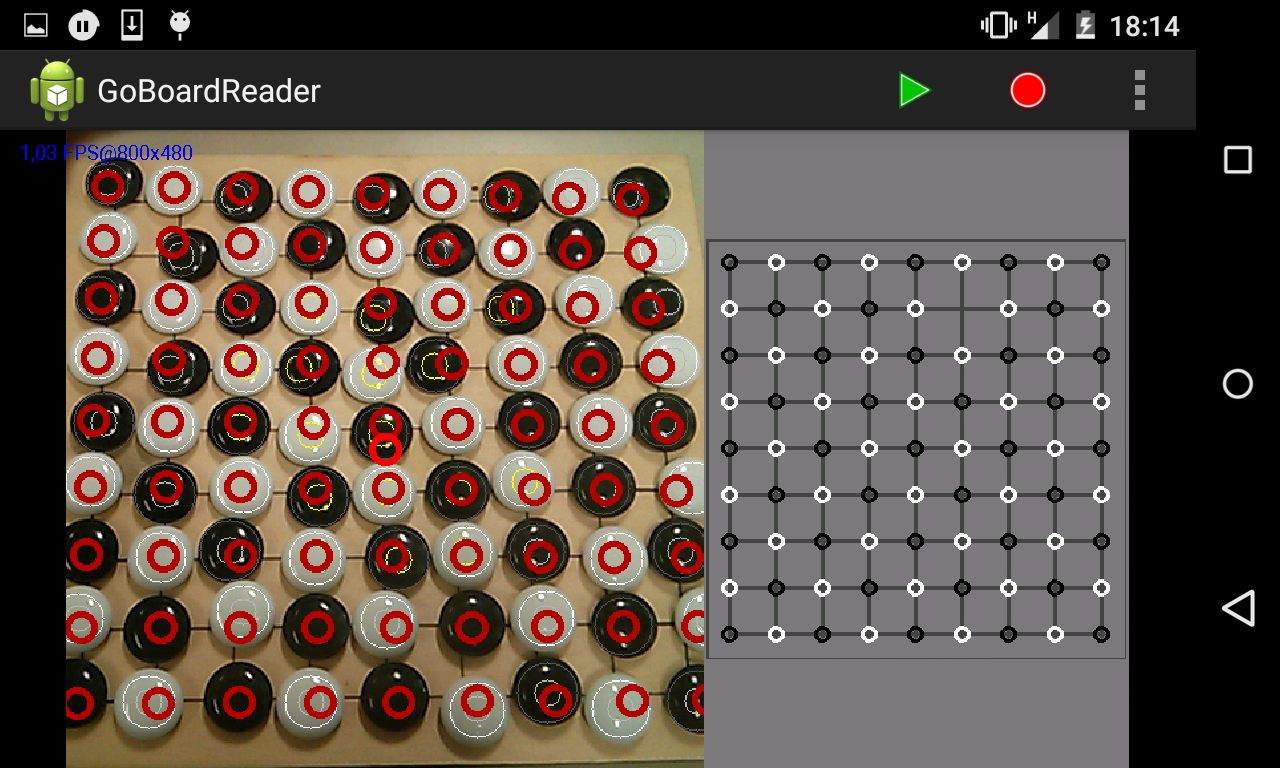
\includegraphics[width=0.7\textwidth]{images/android_perfect_recognition.png}
		\caption{The performance on a hand-held Nexus 4 and a completely covered board}
		\label{fig:android_perfect_recognition}
	\end{figure}
	Two more games were played under difficult lighting conditions in an inner courtyard. The opening in the ceiling cast large reflections on the black stones and strong winds shook the camera. In total there were three pieces which were not detected persistently, i.e. they vanished and reappeared several times. Two pieces were not detected at all. One move was detected too late and there were two false positives. Under these difficult conditions 90.3\% of all pieces on the board were detected correctly.

	Lastly we recreated a game on a desk near a window under neon lighting. Here we encountered one piece which was not detected persistently and one which was not detected at all. That makes a 93.8\% detection ratio. Also there was one false positive at the very end of the game, after both players had passed.

	After this we tried to max out the amount of pieces we could place on the board to see how well the algorithm performed under extreme circumstances. The result was pretty good. Detection was possible until the board was nearly completely covered in pieces. We then put a piece on each intersection in a checkerboard like pattern -- alternating black and white. Even this completely abnormal configuration could be detected with near 100\% accuracy as \autoref{fig:android_perfect_recognition} shows. The results were very unstable, though. That means between a correctly classified frame lay several discarded ones, which did not contribute to the detection result but prolonged the detection time. Of course this is not a valid state of a game of Go, but it goes to show the power of using intersections when detecting densely occupied boards.
